\documentclass{ctexart}
\title{系统开发工具基础第一次实验报告}
\author{张烨 23020007162}
\date{\today}
\usepackage{graphicx}
\usepackage{float}
\graphicspath{{figures/}}
\bibliographystyle{plain}
\usepackage{xltxtra}
\ctexset{
	section={
		%format用于设置章节标题全局格式,作用域为标题和编号
		%字号为小三,字体为黑体,左对齐
		%+号表示在原有格式下附加格式命令
		format+ = \zihao{-3} \heiti \raggedright,
		%name用于设置章节编号前后的词语
		%前、后词语用英文状态下,分开
		%如果没有前或后词语可以不填
		name = {,、},
		%number用于设置章节编号数字输出格式
		%输出section编号为中文
		number = \chinese{section},
		%beforeskip用于设置章节标题前的垂直间距
		%ex为当前字号下字母x的高度
		%基础高度为1.0ex,可以伸展到1.2ex,也可以收缩到0.8ex
		beforeskip = 1.0ex plus 0.2ex minus .2ex,
		%afterskip用于设置章节标题后的垂直间距
		afterskip = 1.0ex plus 0.2ex minus .2ex,
		%aftername用于控制编号和标题之间的格式
		%\hspace用于增加水平间距
		aftername = \hspace{0pt}
	},
	subsection={
		format+ = \zihao{4} \kaishu \raggedright,
		%仅输出subsection编号且为中文
		number = \chinese{subsection},
		name = {(,)},
		beforeskip = 1.0ex plus 0.2ex minus .2ex,
		afterskip = 1.0ex plus 0.2ex minus .2ex,
		aftername = \hspace{0pt}
	},
	subsubsection={
		%设置对齐方式为居中对齐
		format+ = \zihao{-4} \fangsong \centering,
		%仅输出subsubsection编号,格式为阿拉伯数字,打字机字体
		number = \ttfamily\arabic{subsubsection},
		name = {,.},
		beforeskip = 1.0ex plus 0.2ex minus .2ex,
		afterskip = 1.0ex plus 0.2ex minus .2ex,
		aftername = \hspace{0pt}
	}
}
\begin{document}
	\maketitle
	\tableofcontents
	\newpage
	\section{实验目的}
	1.学习版本控制(Git)
	
	通过学习课程资料和课下的一些自主学习,能够掌握基本的Git指令,通过不断学习,继续强化。
	
	2.学习LaTeX文档编辑
	
	学习LaTeX文档编辑器,掌握LaTeX的排版方法,能够用LaTeX来生成自己的实验报告。
	\section{实验内容}
	\subsection{Git}
	\subsubsection{创建本地空仓库}
	创建本地仓库的条件是需要一个空目录,然后在空目录中初始化你的项目
	
	比如说我想要创建一个名为"mytest"的空项目:
	
	1.创建目录
	\begin{figure}[H]
		\centering
		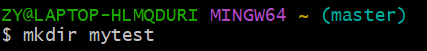
\includegraphics{mkdir}
		\caption{mkdir}
	\end{figure}
	
	2.进入目录
	\begin{figure}[H]
		\centering
		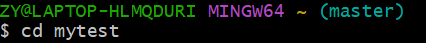
\includegraphics{cd}
		\caption{cd}
	\end{figure}
	
	3.使用git init初始化当前仓库
	\begin{figure}[H]
		\centering
		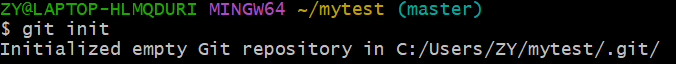
\includegraphics{git init}
		\caption{git init}
	\end{figure}
	
	\subsubsection{添加和提交文件}
	首先我们要知道Git的本地数据管理分为三个区域,分别是工作区,暂存区和本地仓库,而文件只有被放进暂存区才能通过git commit添加进仓库
	
	1.git status
	
    用于显示当前git仓库的状态信息
	
	例如:
	
	工作目录和暂存区的修改情况
	
	哪些文件已被修改但尚未暂存
	
	哪些文件已被暂存但尚未提交
	
	当前分支的状态和与远程分支的差异
	\begin{figure}[H]
		\centering
		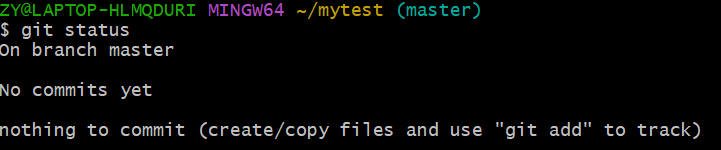
\includegraphics{git status}
		\caption{git status}
	\end{figure}
	
	2.echo
	
	在此我们使用echo创建文件并写入内容
	
	3.git add 该命令用于将用于将文件添加到暂存区
	
	常见的有:
	
	git add 文件名+文件类型
	
	eg:git add file1.txt
	
	git add *.txt  当文件较多时 这个命令可以把所有的txt文件都放入暂存区
	
	git add . 这个可以把所有文件都放入暂存区
	
	4.git commit/git commit -m
	
	git commit -m 描述 ,-m后面的内容是提交的信息用于描述这次提交的目的或内容
	
	eg: git commit -m "这是第一次提交“
	
	当然也可以不用-m 直接用 git commit 这时候就会跳转到一个页面 先输入i才能进入编辑模式 然后可以写这是第一次提交 然后点Esc输入:wq就可以保存退出了
	\begin{figure}[H]
		\centering
		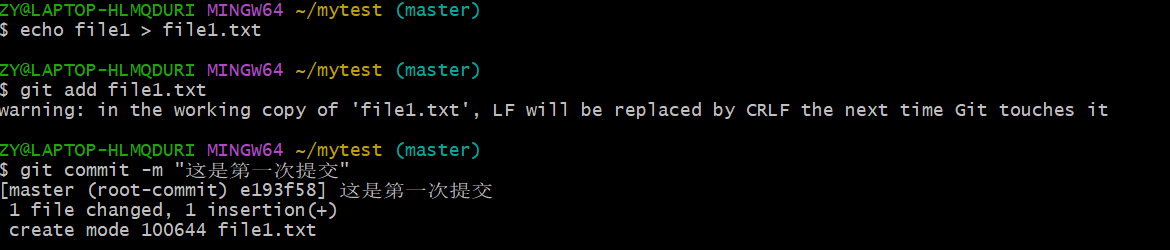
\includegraphics[scale=0.5]{1}
		\caption{关于文件}
	\end{figure}
	
	
	\subsubsection{查看提交历史}
	
	在此,多写几个文件便于查看
	\begin{figure}[H]
		\centering
		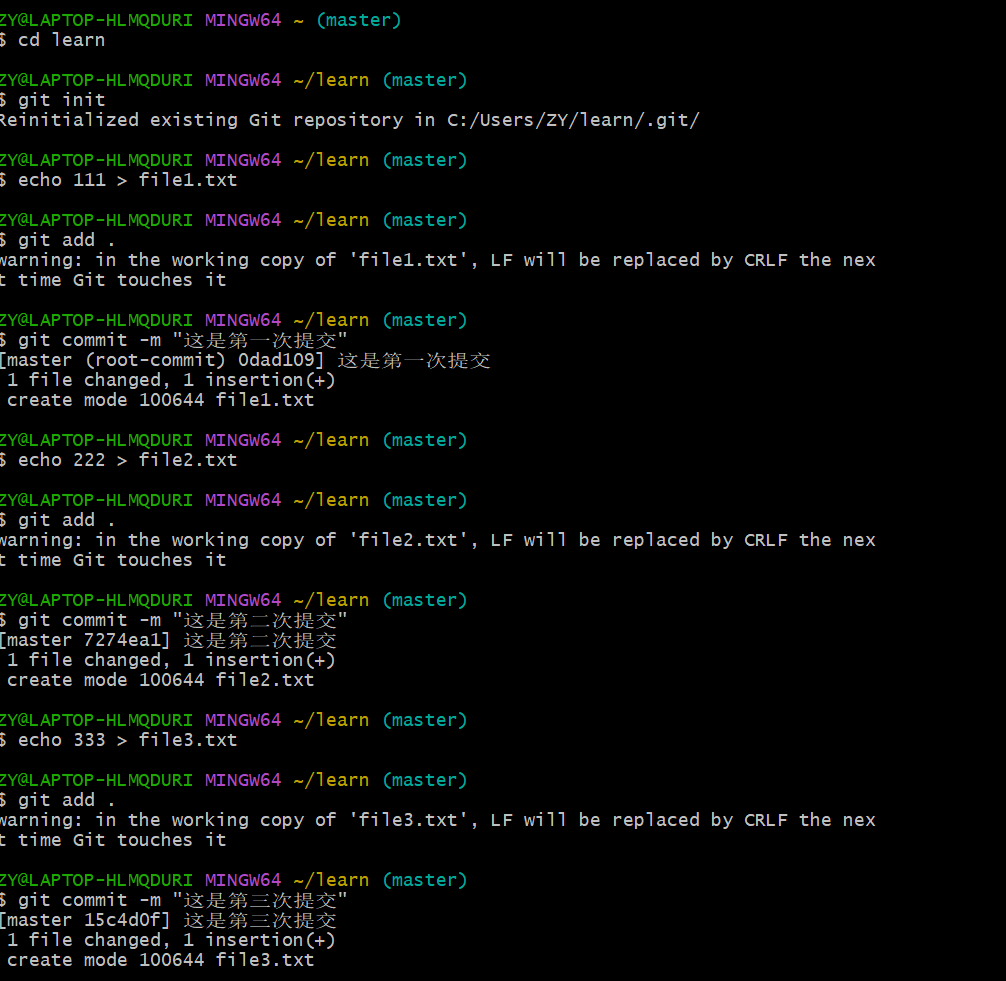
\includegraphics[scale=0.5]{2}
		\caption{添加文件}
	\end{figure}
	
	1.git log 是一个用于查看 Git 仓库提交历史的命令。运行它会列出所有的提交记录,从最新的提交开始,显示每个提交的哈希值、作者、日期和提交信息
	\begin{figure}[H]
		\centering
		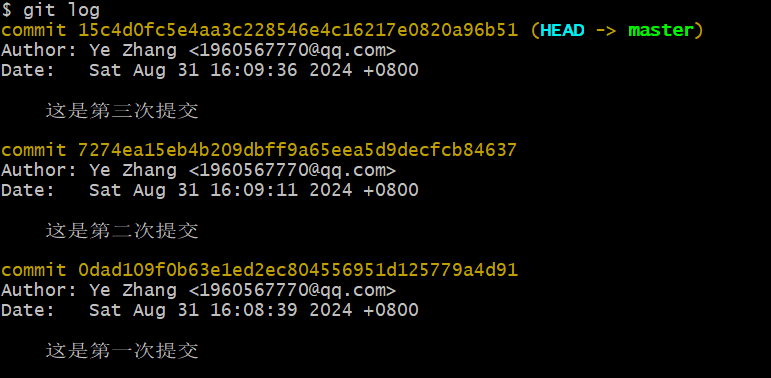
\includegraphics[scale=0.5]{3}
		\caption{git log}
	\end{figure}
	
	2.其他:
	
	git log --oneline:以简洁的单行格式显示每个提交
	\begin{figure}[H]
		\centering
		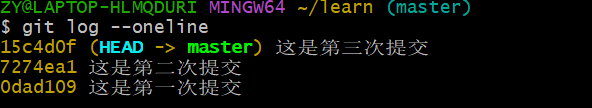
\includegraphics{4}
		\caption{git log --oneline}
	\end{figure}
	
	git log --graph:以图形化形式展示分支和合并历史
	\begin{figure}[H]
		\centering
		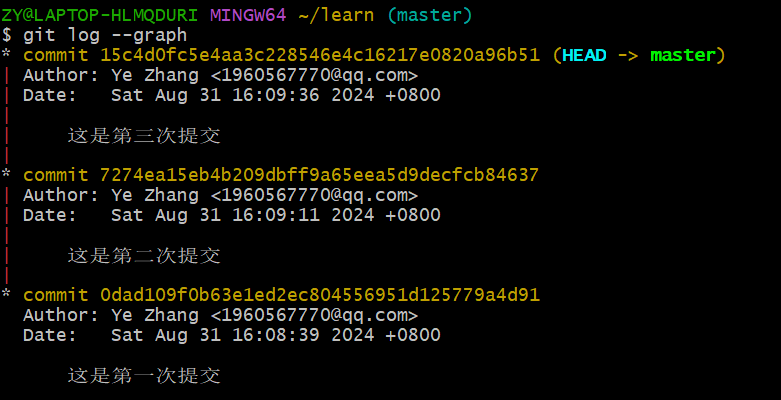
\includegraphics[scale=0.5]{5}
		\caption{git log --graph}
	\end{figure}
	
	git log -p:显示每个提交的差异
	\begin{figure}[H]
		\centering
		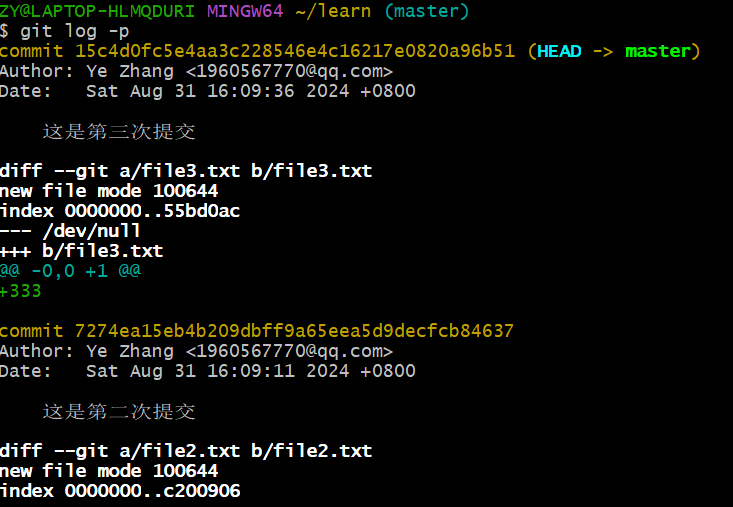
\includegraphics[scale=0.5]{6}
		\caption{git log --p}
	\end{figure}
	
	git log -n :只显示最近的n个提交
	\begin{figure}[H]
		\centering
		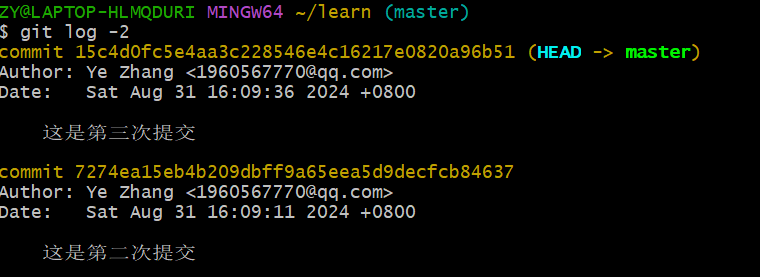
\includegraphics{7}
		\caption{git log --n}
	\end{figure}
	
	git log --oneline --graph --decorate:以简洁的格式和图形化展示提交历史,并包含分支和标签信息
	\begin{figure}[H]
		\centering
		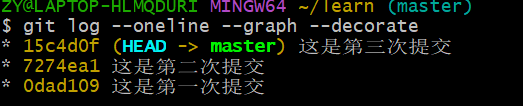
\includegraphics{8}
		\caption{git log --oneline --graph --decorate}
	\end{figure}
	
	\subsubsection{给git log --oneline --graph --decorate起别名graph}
	
	打开.gitconfig,
	\begin{figure}[H]
		\centering
		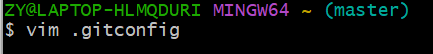
\includegraphics{9}
		\caption{打开}
	\end{figure}
	
	添加:
	 
	[alias]
	graph = log --all --graph --decorate --oneline
	\begin{figure}[H]
		\centering
		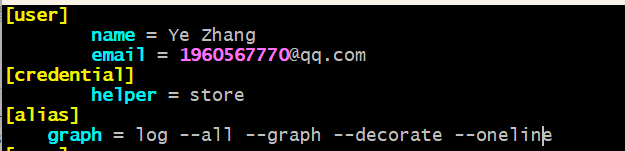
\includegraphics{10}
		\caption{graph}
	\end{figure}
	
	\subsubsection{将本地仓库与远程仓库连接起来}
	
	首先我们在GitHub上创建一个仓库
	\begin{figure}[H]
		\centering
		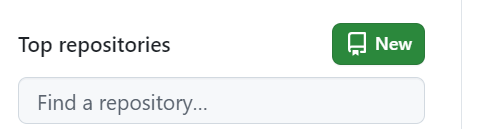
\includegraphics{12}
		\caption{创建仓库}
	\end{figure}
	然后使用git remote add origin HTTPS/SSH,在此,我使用的是SSH
	\begin{figure}[H]
		\centering
		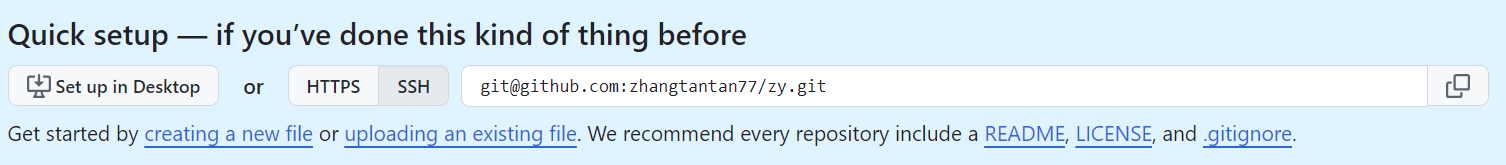
\includegraphics{13}
		\caption{复制地址}
	\end{figure}
	
	\begin{figure}[H]
		\centering
		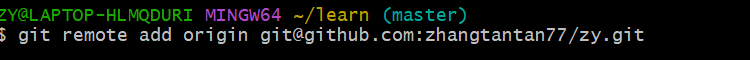
\includegraphics{14}
		\caption{连接}
	\end{figure}
	
	\subsubsection{将本地文件添加进远程仓库}
	在learn仓库中,之前已经添加了三个文件,我们使用ls命令查看
	\begin{figure}[H]
		\centering
		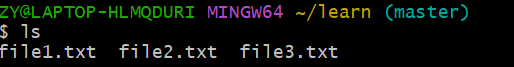
\includegraphics{16}
		\caption{显示文件和目录的名称}
	\end{figure}
	
	我们使用git push命令将这三个文件添加进远程仓库
	\begin{figure}[H]
		\centering
		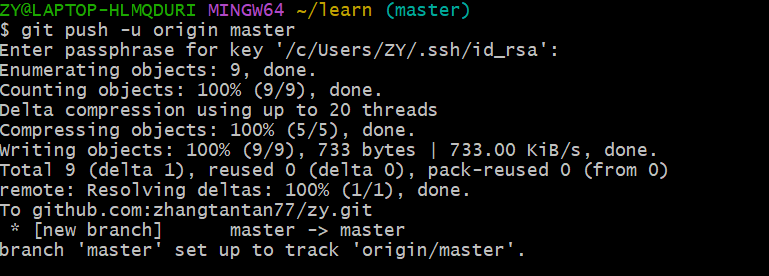
\includegraphics{17}
		\caption{添加进远程仓库}
	\end{figure}
	
	然后刷新一下,就可以看到仓库中出现了这三个文件
	\begin{figure}[H]
		\centering
		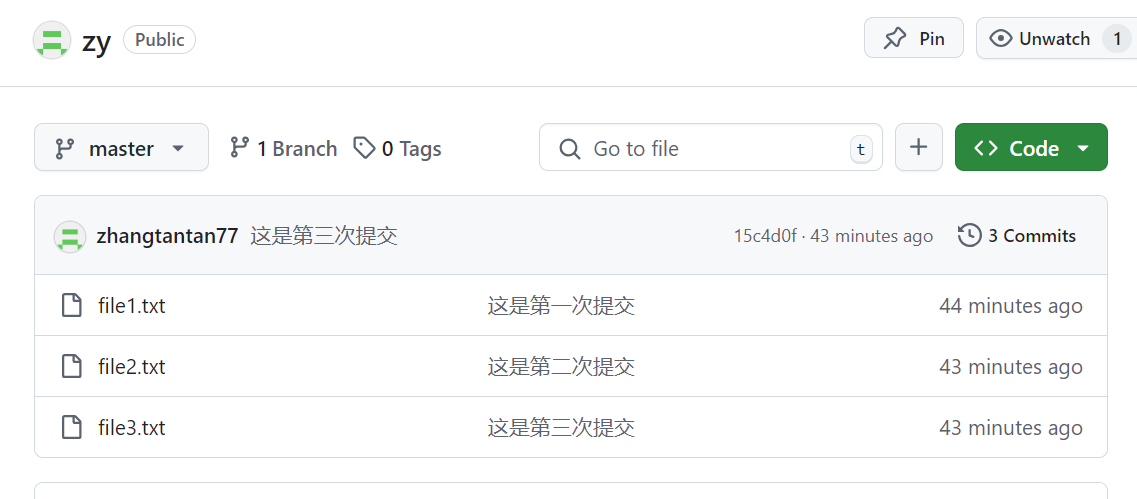
\includegraphics[scale=0.5]{15}
		\caption{仓库}
	\end{figure}
	
	\subsubsection{克隆GitHub上的仓库}
	在此我克隆的是之前自己在GitHub上创建过的一个仓库remote-repo
	\begin{figure}[H]
		\centering
		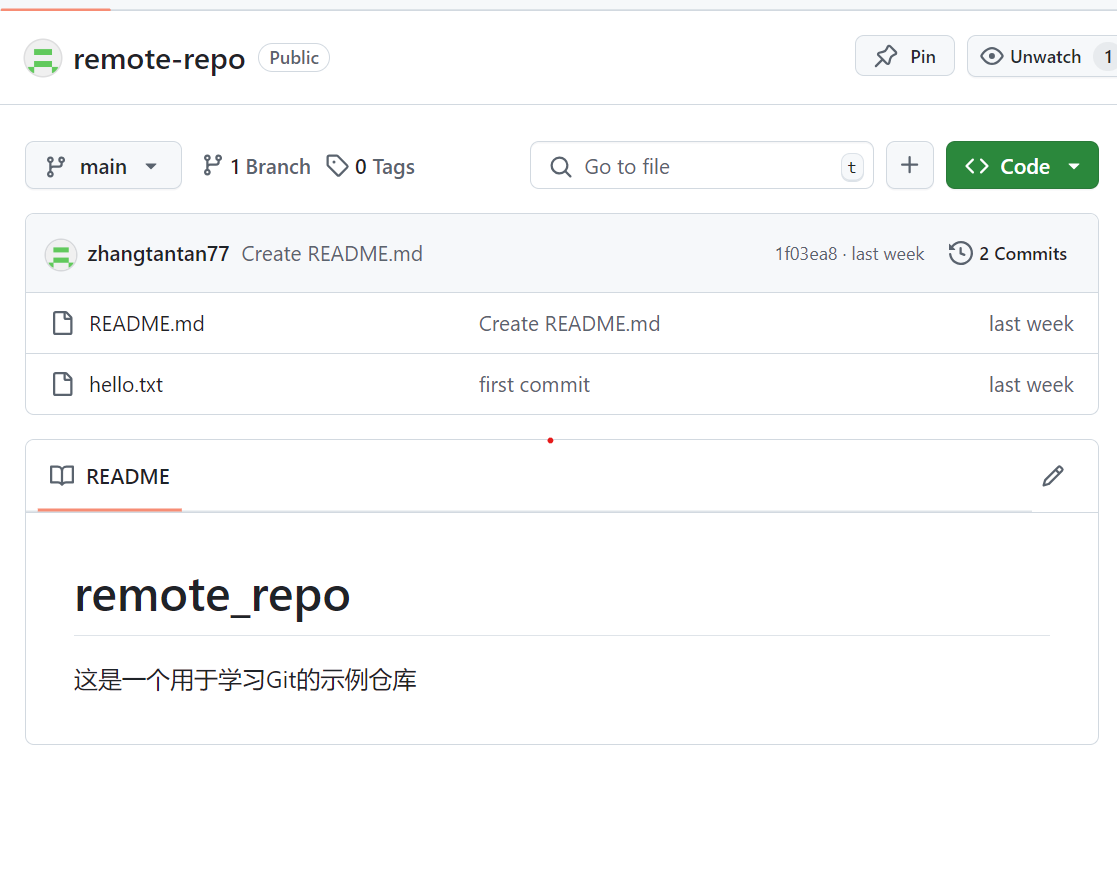
\includegraphics[scale=0.5]{23}
		\caption{remote-repo仓库}
	\end{figure}
	点击绿色的code,然后复制SSHSH
	\begin{figure}[H]
		\centering
		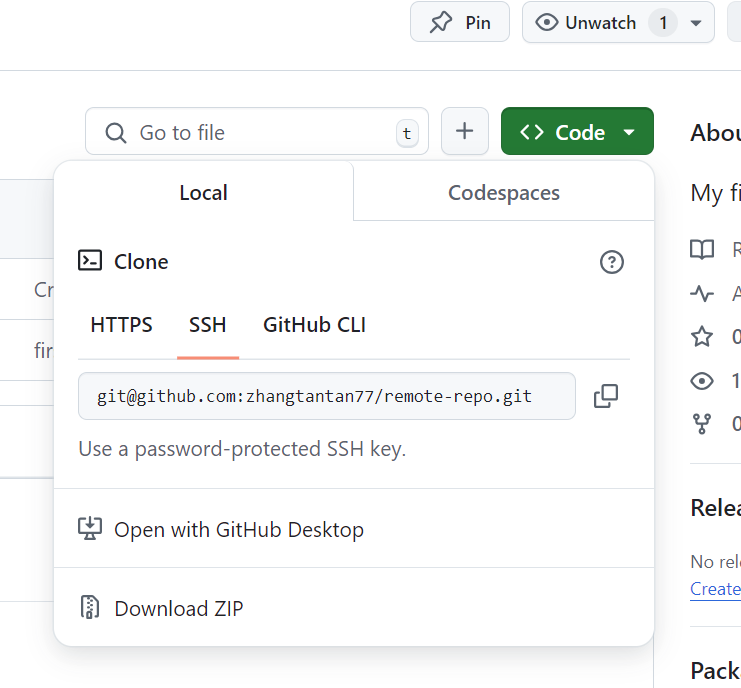
\includegraphics{24}
		\caption{复制}
	\end{figure}
	git clone SSH
	\begin{figure}[H]
		\centering
		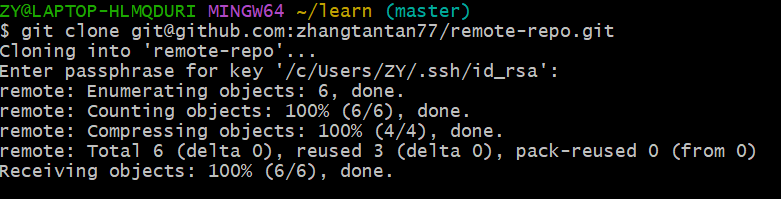
\includegraphics{25}
		\caption{克隆}
	\end{figure}
	
	因为我之前设置过SSH,所以需要输入密码
	
	打开learn仓库所在目录,就可以看见learn目录下除了之前的三个文件,还有remote-repo
	
	\begin{figure}[H]
		\centering
		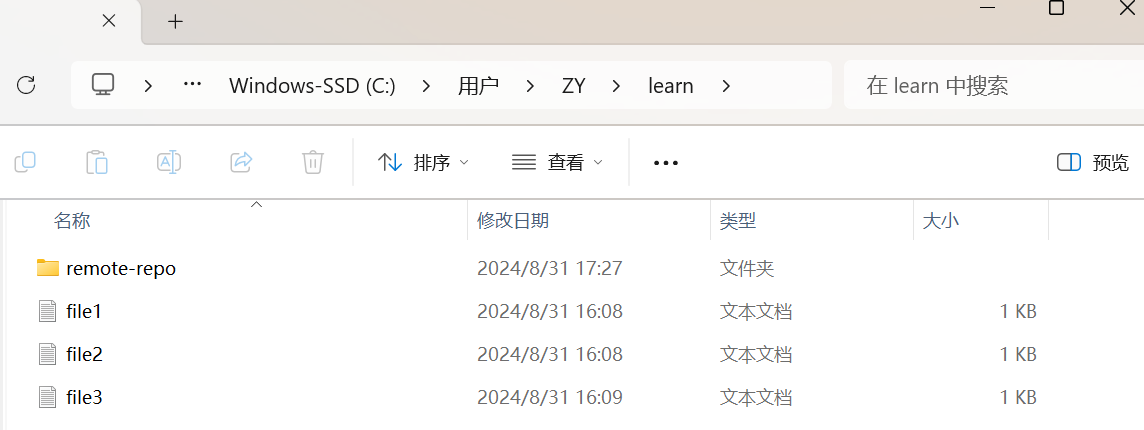
\includegraphics{26}
		\caption{成功}
	\end{figure}
	
	\subsubsection{修改远程仓库上的内容}
	现在我们要修改remote-repo中的内容,先前可以看到,remote-repo中有hello.txt文件,打开hello.txt可以看到原来的内容是hello
	\begin{figure}[H]
		\centering
		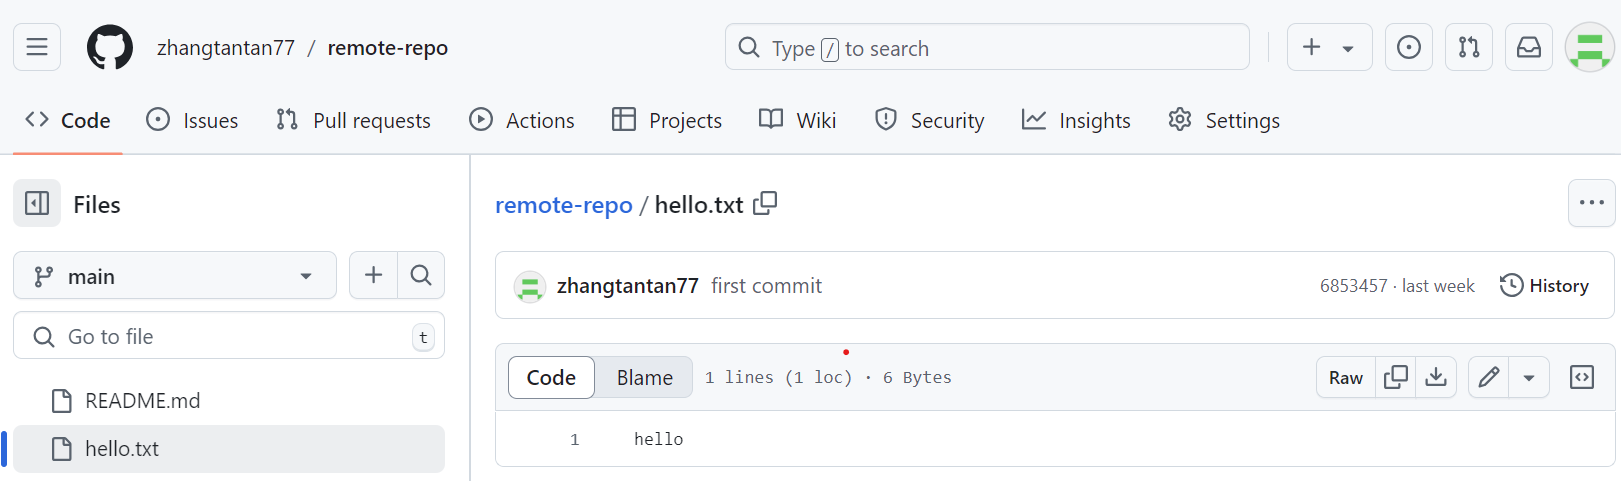
\includegraphics[scale=0.5]{27}
		\caption{hello}
	\end{figure}
	
	现在我们想把原来的内容替换成11111
	
	首先cd remote-repo,进入当前目录
	
	然后使用echo命令修改内容
	
	再使用git add和git commit命令,最后使用git push命令推送给远程仓库
	
	\begin{figure}[H]
		\centering
		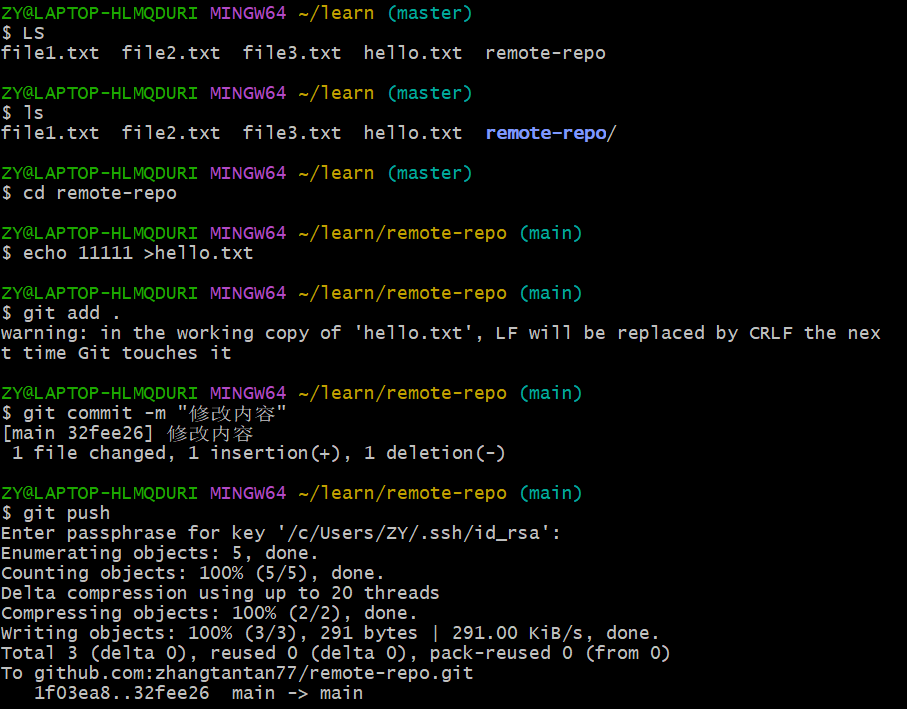
\includegraphics[scale=0.5]{28}
		\caption{修改}
	\end{figure}
	
	任何刷新一下就可以看到修改成功
	\begin{figure}[H]
		\centering
		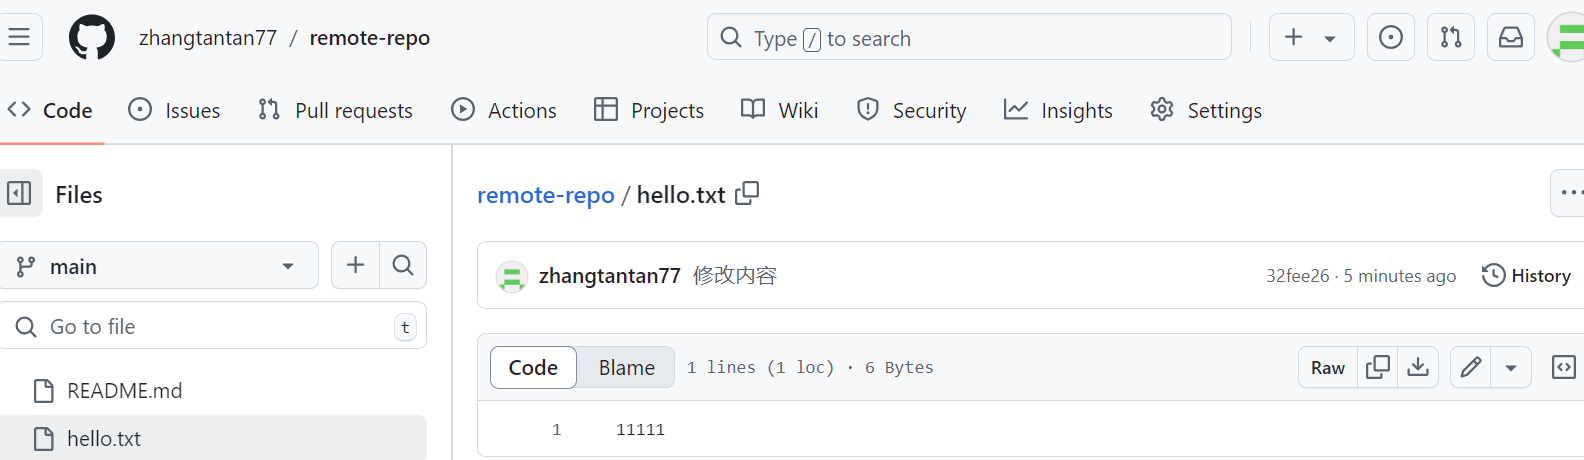
\includegraphics[scale=0.5]{29}
		\caption{成功}
	\end{figure}
	
	\subsubsection{删除文件}
	git rm 文件 
	
	该命令把文件从工作区和暂存区同时删除,要注意提交,否则删除的文件在版本库中还是存在的,在这里我们删除file1.txt
	
	\begin{figure}[H]
		\centering
		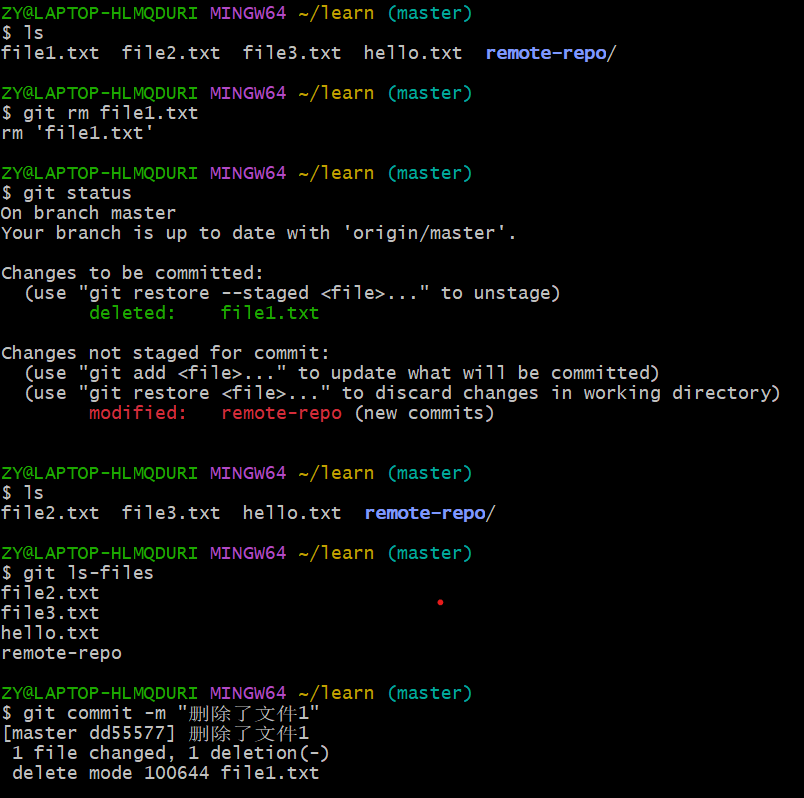
\includegraphics[scale=0.5]{30}
		\caption{删除文件}
	\end{figure}
	
	\subsubsection{git reset 回退版本的三种命令}
	在此新建一个仓库repo,并分三次添加三个文件
	\begin{figure}[H]
		\centering
		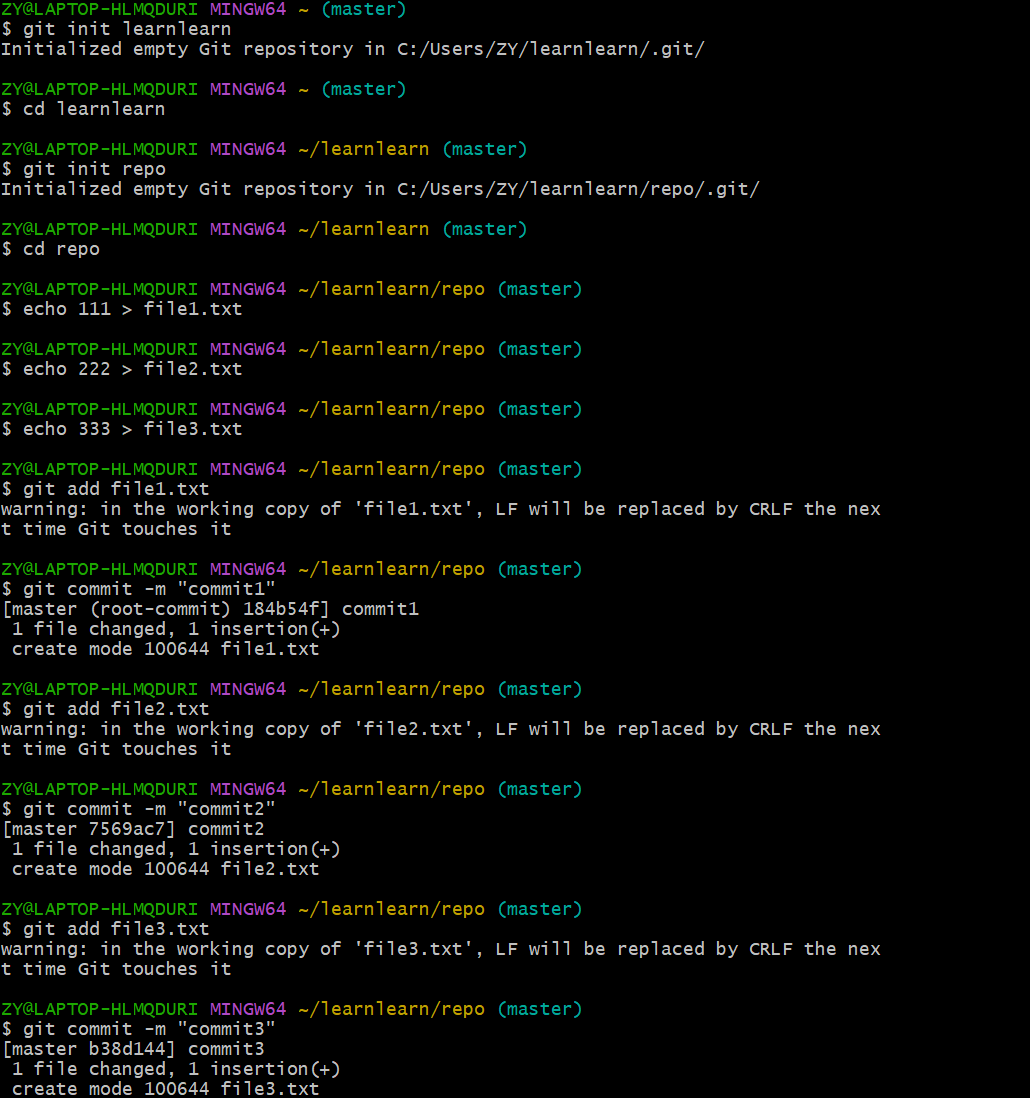
\includegraphics[scale=0.3]{33}
		\caption{新建}
	\end{figure}
	
	为了方便比较,将仓库目录复制三份
	\begin{figure}[H]
		\centering
		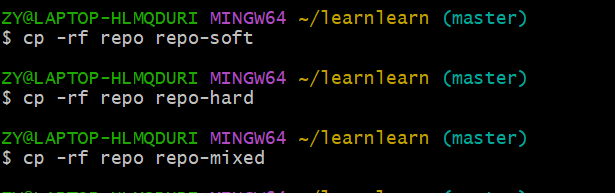
\includegraphics{34}
		\caption{复制}
	\end{figure}
	
	1.git reset --soft 表示回退到某一个版本,并且保留工作区和暂存区的所有修改内容
	\begin{figure}[H]
		\centering
		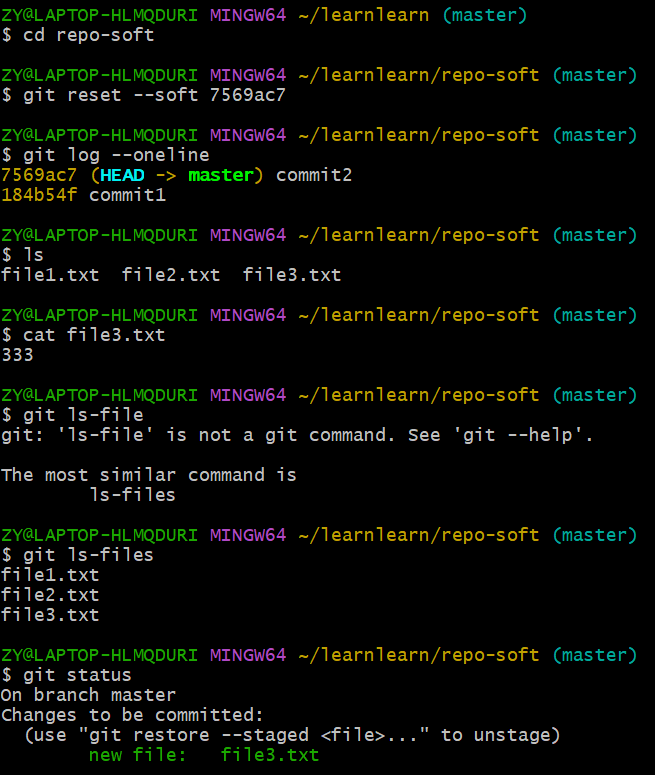
\includegraphics[scale=0.5]{35}
		\caption{soft}
	\end{figure}
	
	2.git reset --hard 表示回退到某一个版本,并且丢弃工作区和暂存区的所有修改内容
	\begin{figure}[H]
		\centering
		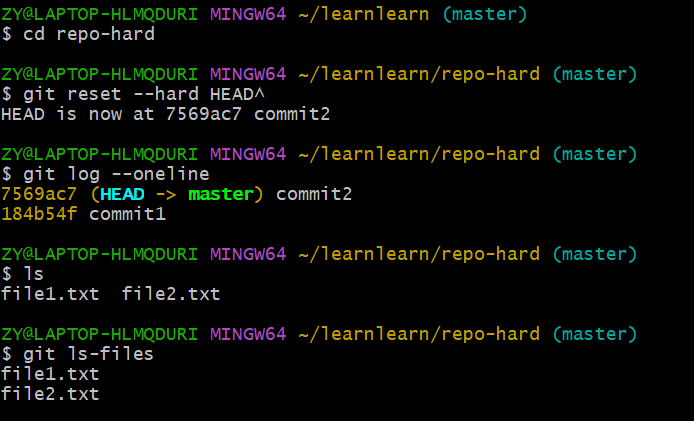
\includegraphics[scale=0.5]{36}
		\caption{hard}
	\end{figure}
	
	3.git reset --mixed 表示回退到某一个版本,并且只保存工作区的修改内容
	\begin{figure}[H]
		\centering
		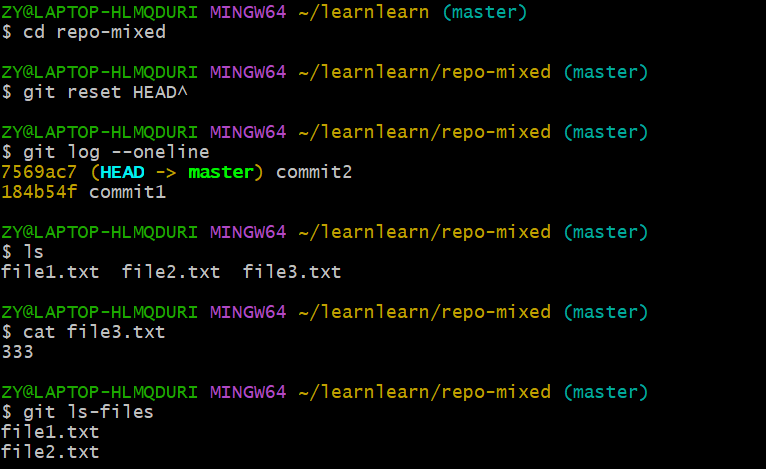
\includegraphics[scale=0.5]{37}
		\caption{mixed}
	\end{figure}
	
	\subsection{LaTeX}
	\subsubsection{LaTeX中的文章结构}
	LaTeX中的文章分为导言区和正文区
	
	导言区:
	
	\verb|\documentclass{article}|
	
    使用documentclass引入文档类,此外还有book类,report类,letter类
    
    标题:
    
    \verb|\title{my first article}|
    
    作者:
    
    \verb|\author{tantan}|
    
    日期:
    
    \verb|\date{\today}|
	
	还有一些宏包也都是在导言区
	
	正文区:
	
	\verb|\begin{document}|
		
		内容
		
	\verb|\end{document}|
	
	用begin和end输入一个环境名称,我们设定为document,注意一个latex文件只能有一个document环境
	
	我们使用\verb|\maketitle|输出整个标题
	
	\subsubsection{LaTeX中使用中文}
	为了在LaTeX中使用中文,我们需要在导言区引入一个宏包\verb|\usepackage{ctex}|
	
	还有另一种方法,就是在导言区只写\verb|\documentclass{ctexart}|,对应的其他类为\verb|ctexbook  ctexrep|,注意没有letter对应的
	
	\subsubsection{LaTeX中的数学公式}
	在LaTeX中,我们使用\verb|$|符号进入数学模式,举个例子:
	
	我们使用\verb|$ 1 + 1 = 2 $|来输出这个简单的数学公式
	
	此外还有\verb|$$|符号
	
	要注意的是,两者的差别在于\verb|$|符号表示行内公式,不会换行,\verb|$$|符号表示行间公式,会换换行
	
	此外,如果我们想产生自动带编号的行间公式,就要使用equation环境
	
	\verb|\begin{equation}|
		
	\verb|\end{equation}|
	
	下面我使用这个环境写几个自动带编号的数学公式
	
	\begin{equation}
		\sin^2 x + \cos^2 x =1
	\end{equation}
	
	\begin{equation}
		a + b = b + a
	\end{equation}
	
	此外,很多数学公式的实现还需要引入amsmath这个宏包,实现方法是在导言区添加\verb|\usepackage{amsmath}|
	
	\subsubsection{LaTeX中的字体}
	在latex中,一个字体有五种属性 :
	
	字体编码 1.正文字体编码:OT1,T1,EU1等 2.数字字体编码:OML,OMS,OMX等
	
	字体族 1.罗马字体:笔画起始处有装饰 2.无衬线字体:笔画起始处无装饰 3.打字机字体:每个字符宽度相同,又称等宽字体
	
	字体系列 1.粗细 2.宽度
	
	字体形状 1.直立 2.斜体 3.伪斜体 4.小型大写
	
	字体大小
	
	这里我们主要讨论中文
	
	使用\verb|\songti|让后续输出的字体为宋体 
	
	使用\verb|\heiti| 让后续输出的字体为黑体
	
	使用\verb|\fangsong|让后续输出的字体为仿宋
	
	使用\verb|\kaishu|让后续输出的字体为楷书
	
	使用\verb|\texbf|让后续输出的字体为粗体
	
	使用\verb|\textit|让后续输出的字体为斜体
	
	使用\verb|\zihao{}| 来限定字体大小,括号里面填数字
	
	\subsubsection{LaTeX中表格的生成}
	在LaTeX中,我们使用tabular环境来生成表格,举个例子:下面这段代码就可以生成
	
	\begin{figure}[H]
		\centering
		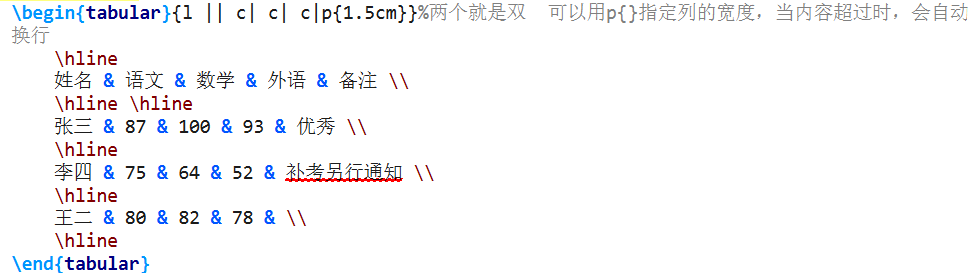
\includegraphics[scale=0.8]{38}
		\caption{表格}
	\end{figure}

	\begin{tabular}{l || c| c| c|p{1.5cm}}%两个就是双  可以用p{}指定列的宽度,当内容超过时,会自动换行
		\hline
		姓名 & 语文 & 数学 & 外语 & 备注 \\
		\hline \hline
		张三 & 87 & 100 & 93 & 优秀 \\
		\hline
		李四 & 75 & 64 & 52 & 补考另行通知 \\
		\hline
		王二 & 80 & 82 & 78 & \\ 
		\hline
	\end{tabular}
	
	这样的一个表格
	
	\subsubsection{LaTeX中插入图片}
	在LaTeX中插入图片需要使用
	\verb|\usepackage{graphicx}|这个宏包,同时插入图片需要和你的txt文件在一个文件夹下,我的图片都在figures文件夹中,那么就可以添加上
	\verb|\graphicspath{{figures/}}|指定搜索目录
	
	然后在正文区使用\verb|\includegraphics{图片文件名}|就好了,也可以使用\verb|\includegraphics[缩放比例]{图片文件名}|,在[]里面加入缩放比例或者指定的长宽高
	
	下面是相关代码:
	\begin{figure}[H]
		\centering
		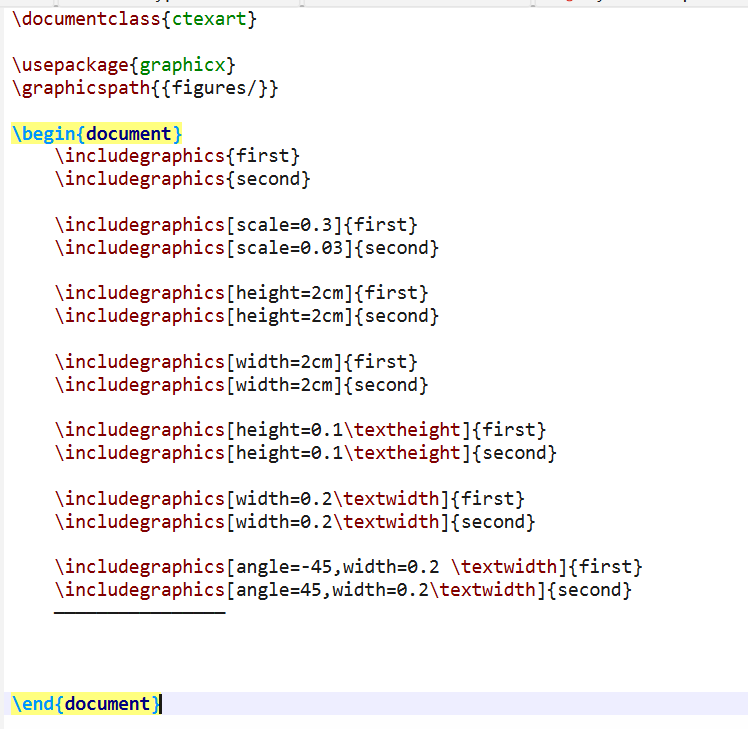
\includegraphics[scale=0.6]{39}
		\caption{插图}
	\end{figure}
	
	\subsubsection{LaTeX中创建章节和子章节}
	在LaTeX中,创建章节一般要用到\verb|\section{}|和\verb|\subsection{}|,\verb|\subsubsection{}|下面是一个简单例子的代码:
	
	\verb|\section{引言}|
	
	\verb|\section{实验方法}|
	
	\verb|\section{实验结果}|
	
	\verb|\subsection{数据}|
	
	\verb|\subsection{图表}|
	
	\verb|\subsubsection{实验条件}|
	
	\verb|\subsubsection{实验过程}|
	
	\verb|\subsection{结果分析}|
	
	\verb|\section{结论}|
	
	\verb|\section{致谢}|
	
	实现效果为:
	\begin{figure}[H]
		\centering
		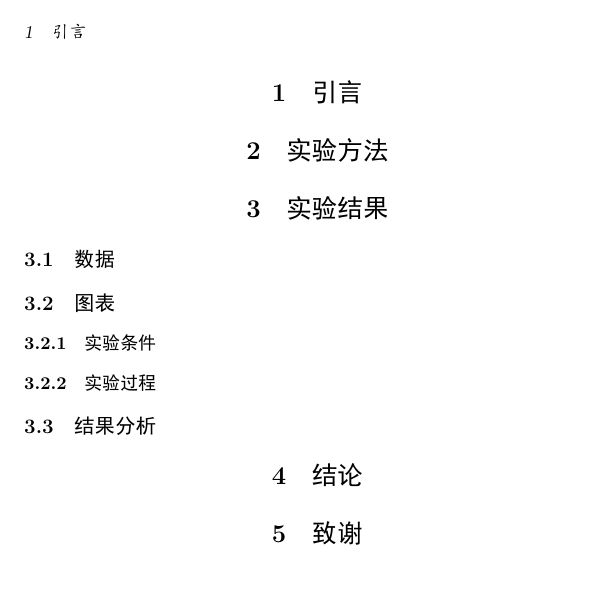
\includegraphics[scale=0.6]{40}
		\caption{章节}
	\end{figure}
	
	\subsubsection{LaTeX中目录的生成}
	在LaTeX中为了自动生成目录,我们需要在正文区添加\verb|\tableofcontents|,通常,为了让目录和后面的正文内容不在同一页,我们可以加上\verb|\newpage|来实现,\verb|\newpage|的作用是另起一页
	
	\subsubsection{LaTeX中书写参考文献}
	在论文的最后,我们需要书写参考文献,在知网上导出我们需要的参考文献,注意选择BibTeX格式,然后新建一个文件,复制进去,注意后缀最好是.bib,在导言区引入\verb|\bibliographystyle{plain}|宏包,然后在最后的正文区加上\verb|\nocite{*}|和\verb|\bibliography{刚才新建的后缀为.bib的文件文件名}|,这里\verb|\notice{*}|的作用是显示我们刚才创建的后缀为.bib文件里面的所以内容,也可以不使用这个命令,每次只添加某条文献,但我感觉这种方法更简单一点,下面我来导入刚才的三个文献:
	\nocite{*}
	\bibliography{text}
	\subsubsection{LaTeX中一些特殊字体的书写}
	比较常见的有:
	
	\verb|\TeX{}|输出\TeX{} 
	
	\verb|\LaTeX{}|输出\LaTeX{}
	
	\verb|\LaTeXe{}|输出\LaTeXe{}
	
	\verb|\XeLaTeX|输出 \XeLaTeX ,不过这个需要在导言区添加\verb|\xltxtra|宏包
	
	\verb|`|表示左单引号`
	
	\verb|'|表示右单引号'
	
	\subsection{心得体会}
	通过学习Git和LaTeX,进一步丰富了自己的技能,同时,在学习过程中也遇到很多问题,但是通过上网查询和同学帮助,最后终于解决了问题。在今后的学习中,我会更加认真,继续提升自己。
	
	\section{相关练习、报告和代码查看链接}
	本次报告相关练习、报告和代码均可以在https://kkgithub.com/zhangtantan77/work查看

\end{document}